\subsection{General}
SpeechVR is a VR application on smartphones: it allows the user to be put into a virtual environment thanks to the usage of only a HMD and the user phone. It also uses a biosensor as a way to manipulate such environment.\\
The application offers two modes to the user:
\begin{itemize}
	\item Free talk;
	\item Interview.
\end{itemize}
The former allows the users to try their own speech while the latter allows them to answer questions sent by other people.

\subsection{Audience}
The audience is divided in three different group: 
\begin{itemize}
	\item Kind classmates \& colleagues: with causal wearing and friendly smile, they will listen with smile, nod and praise the user during the speech.
	\item Indifferent people: with strange clothes, they pay no attention to the speaker and will look around, speak to others and may fall asleep during the speech.
	\item Experts: with formal suit and serious expression, they will listen without emotion, shake head and get angry during the speech.
\end{itemize}

\begin{figure}[H]
	\centering
	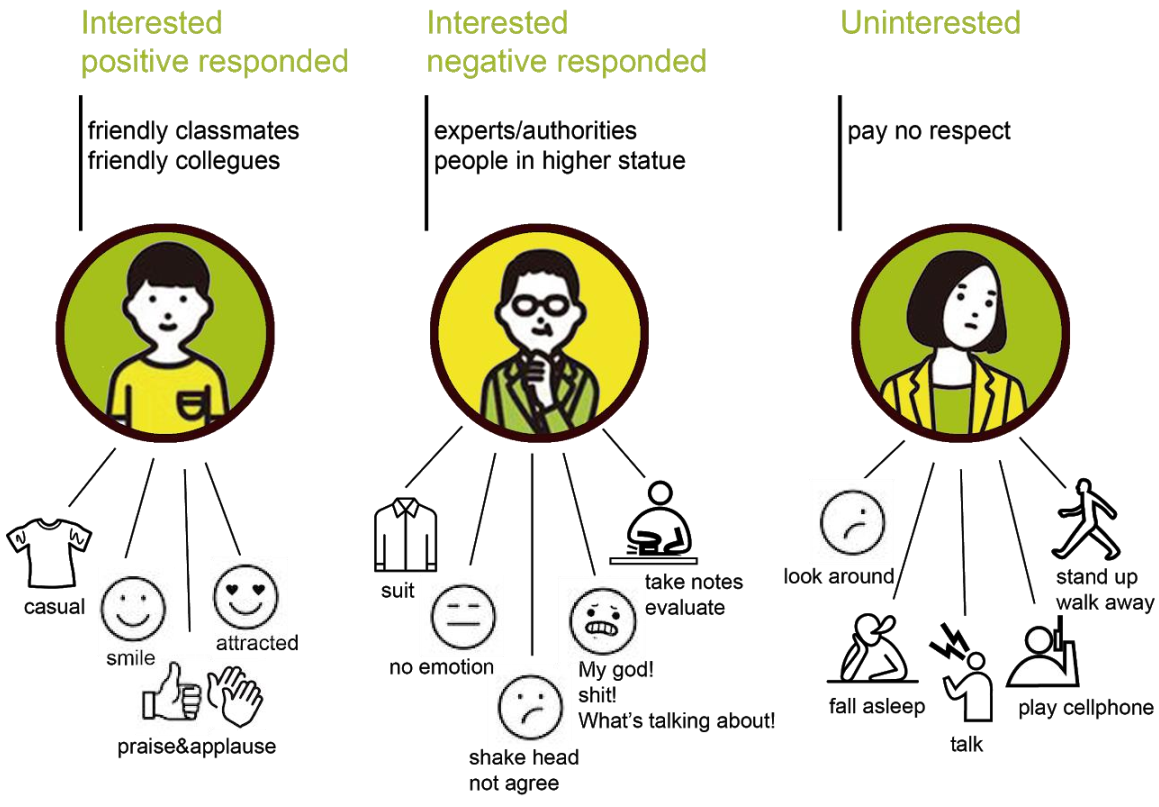
\includegraphics[scale=0.4]{Audience}
	\caption{Audience characteristics}
\end{figure}

The composition of the audience can be chosen before the speech so that the user can choose the challenge he/she want to take on.

\begin{figure}[H]
	\centering
	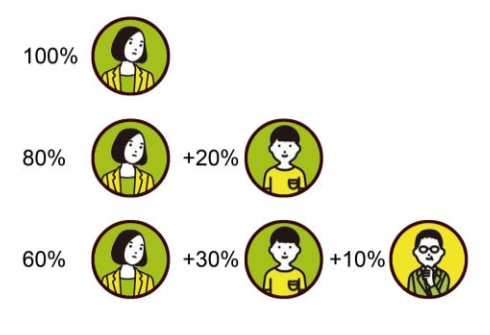
\includegraphics[scale=0.57]{composition2}
	\caption{Example of compositions}
\end{figure}
\subsection{Biosensor}
The biosensor is used as a mean to track the level of anxiety of the user and it allows to manipulate the environment based on the values read:
\begin{itemize}
	\item The number of people in the audience will change throughout the speech. This is achieved by using lights to hide or show more people in the audience;
	\item The speech can be interrupted if the anxiety level determined by the biosensor increased too much.
\end{itemize}
\begin{figure}[H]
	\centering
	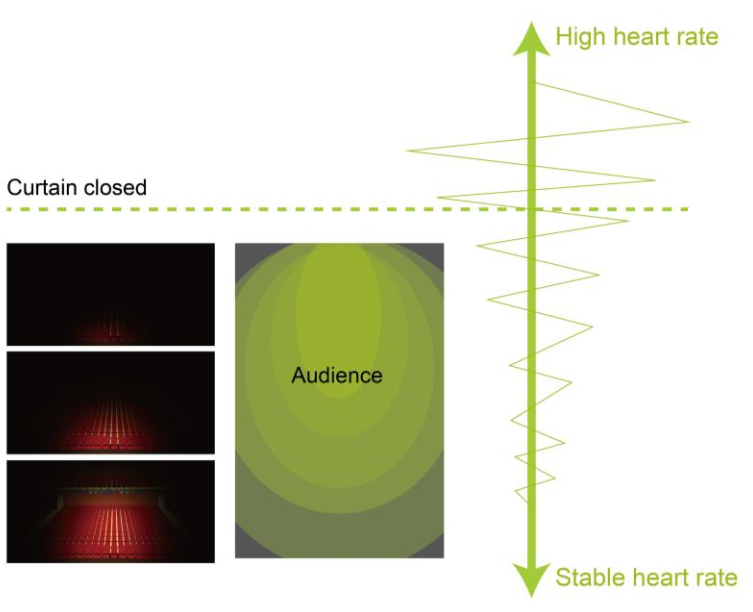
\includegraphics[scale=0.5]{lights}
	\caption{How the lights change based on the biosensor values.}
\end{figure}

\subsection{Process}
The application is divided into three stages:
\begin{itemize}
	\item Menu where the user can decide the settings for the speech:
		\begin{itemize}
			\item Biosensor (through a QR Code scanner)
			\item Speech mode
				\begin{itemize}
					\item Free talk
					\item Interview
				\end{itemize}
			\item Audience composition
		\end{itemize}
	\item Heart rate test where a baseline value for the heart rate is searched: it will be used as reference to determine the state of mind of the user;
	\item VR activity where the user is put into the virtual environment he/she can try the speech.
\end{itemize}

\begin{figure}[H]
	\centering
	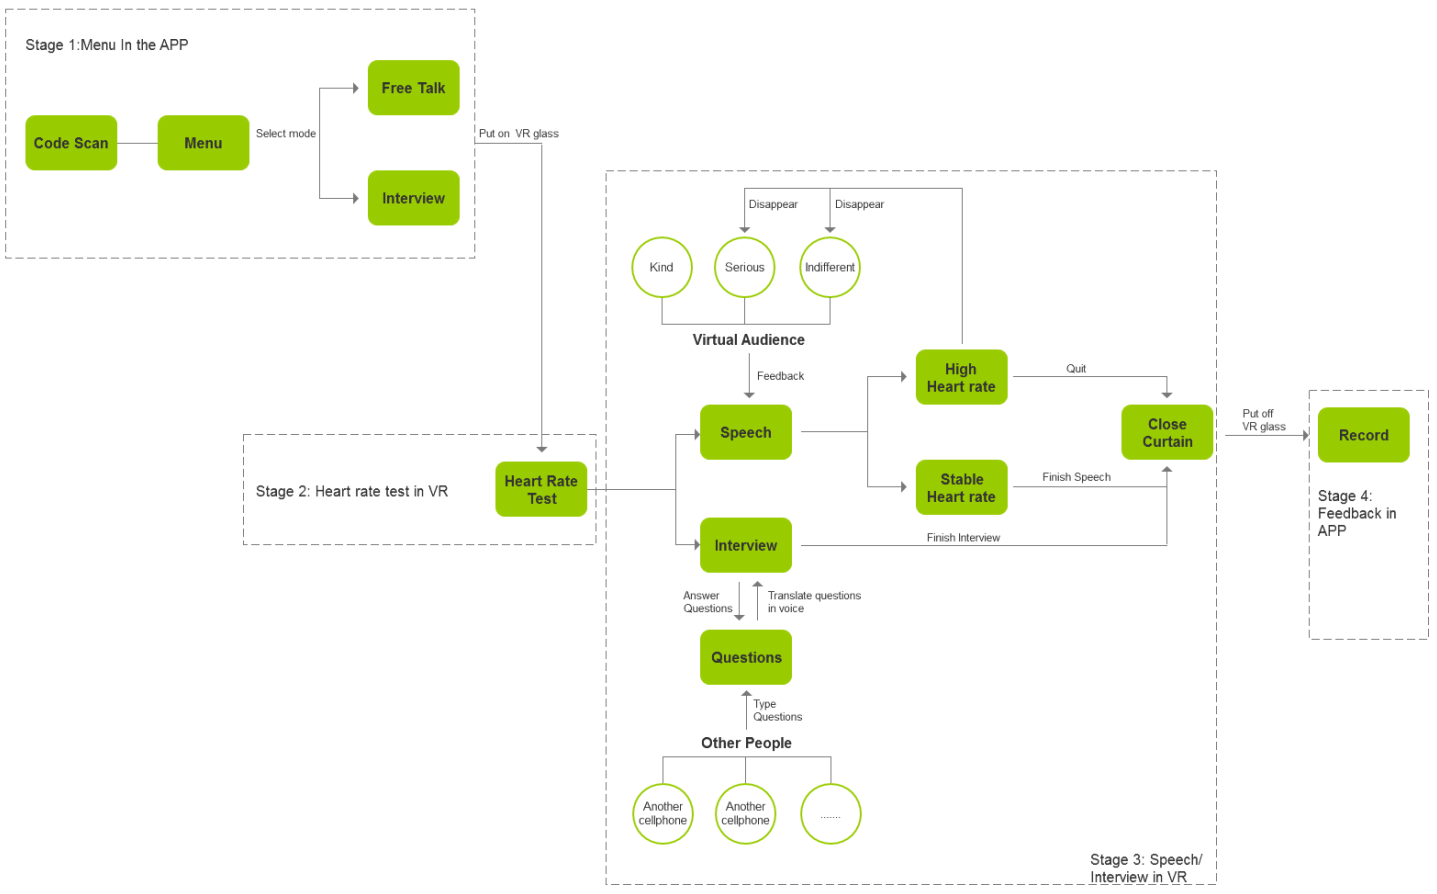
\includegraphics[scale=0.434]{Process}
	\caption{Flow of the application}
\end{figure}


\subsection{Interface}
\begin{figure}[H]
	\centering
	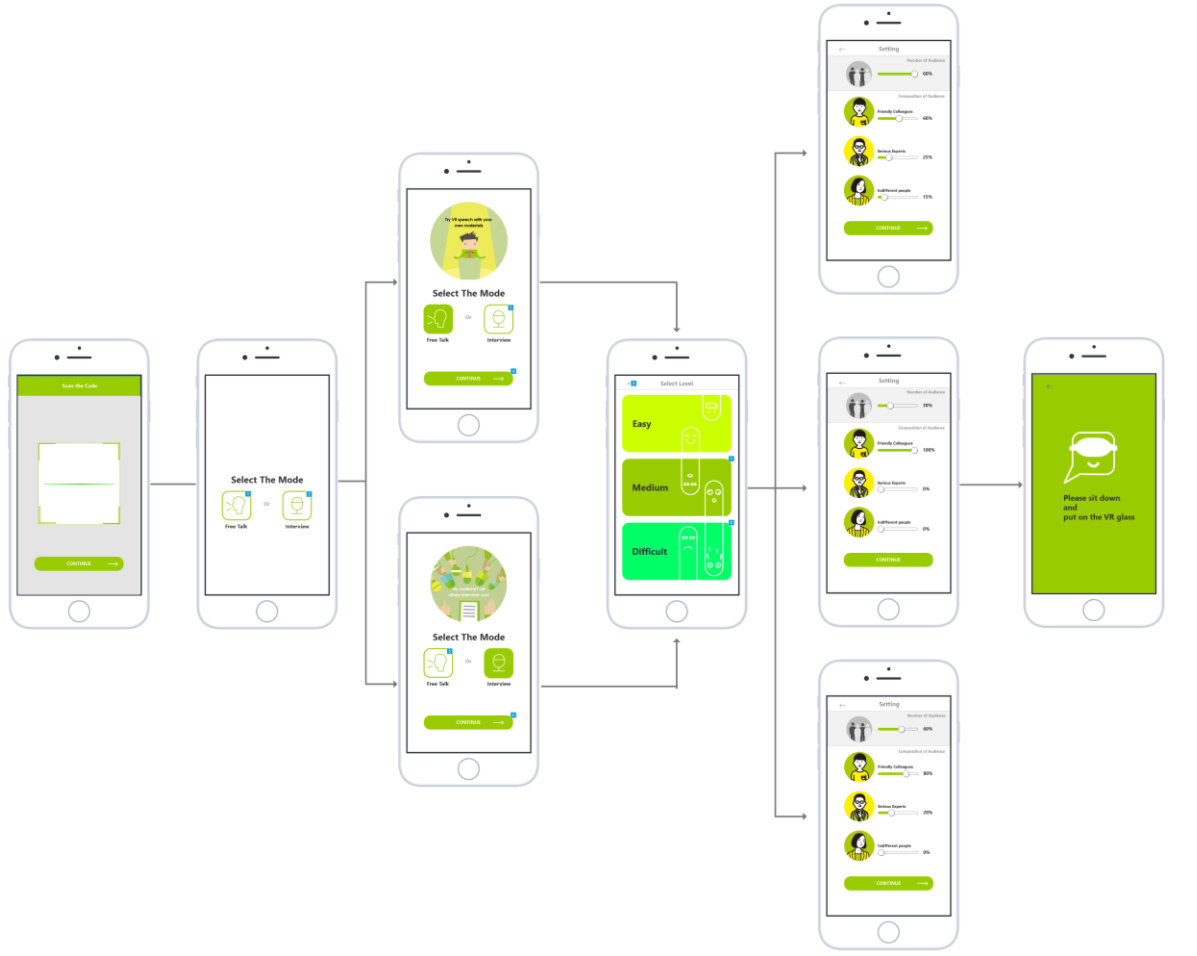
\includegraphics[scale=0.521]{Interface}
	\caption{Stage 1: App}
\end{figure}

\begin{figure}[H]
	\centering
	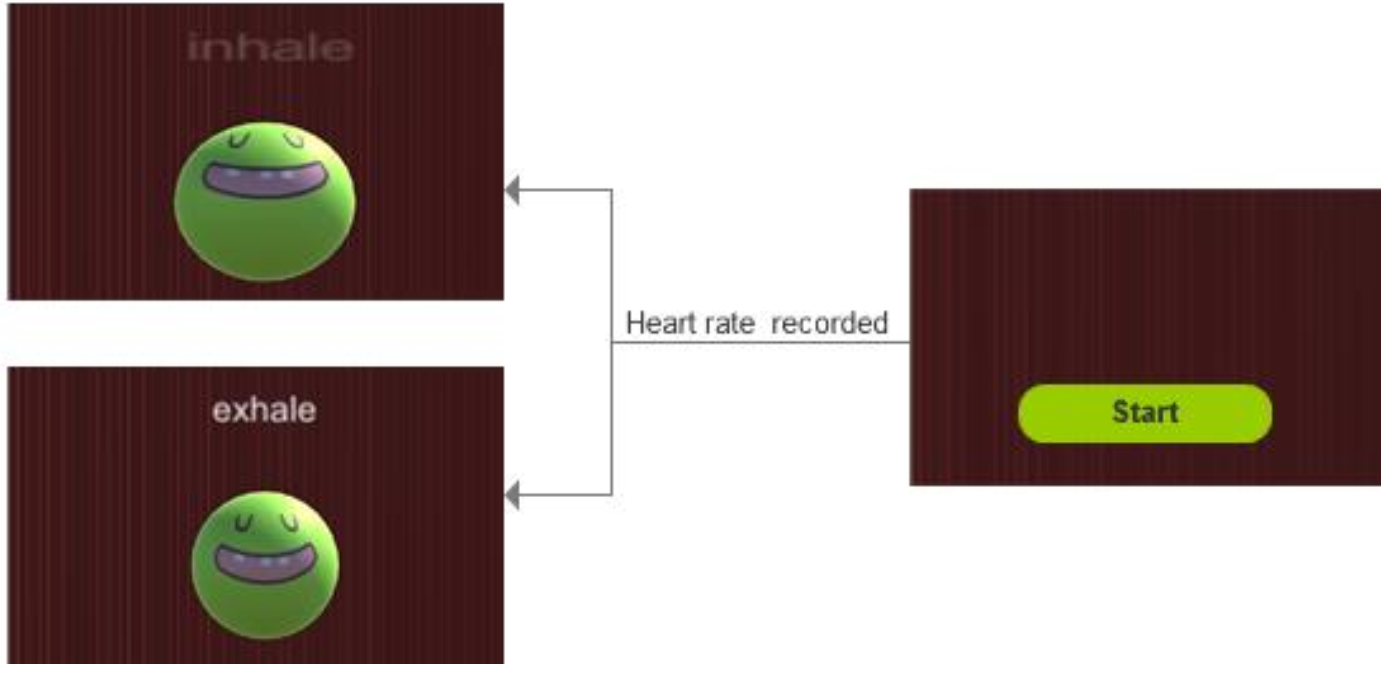
\includegraphics[scale=0.35]{Breathing}
	\caption{Stage 2: Heart rate test}
\end{figure}

\begin{figure}[H]
	\centering
	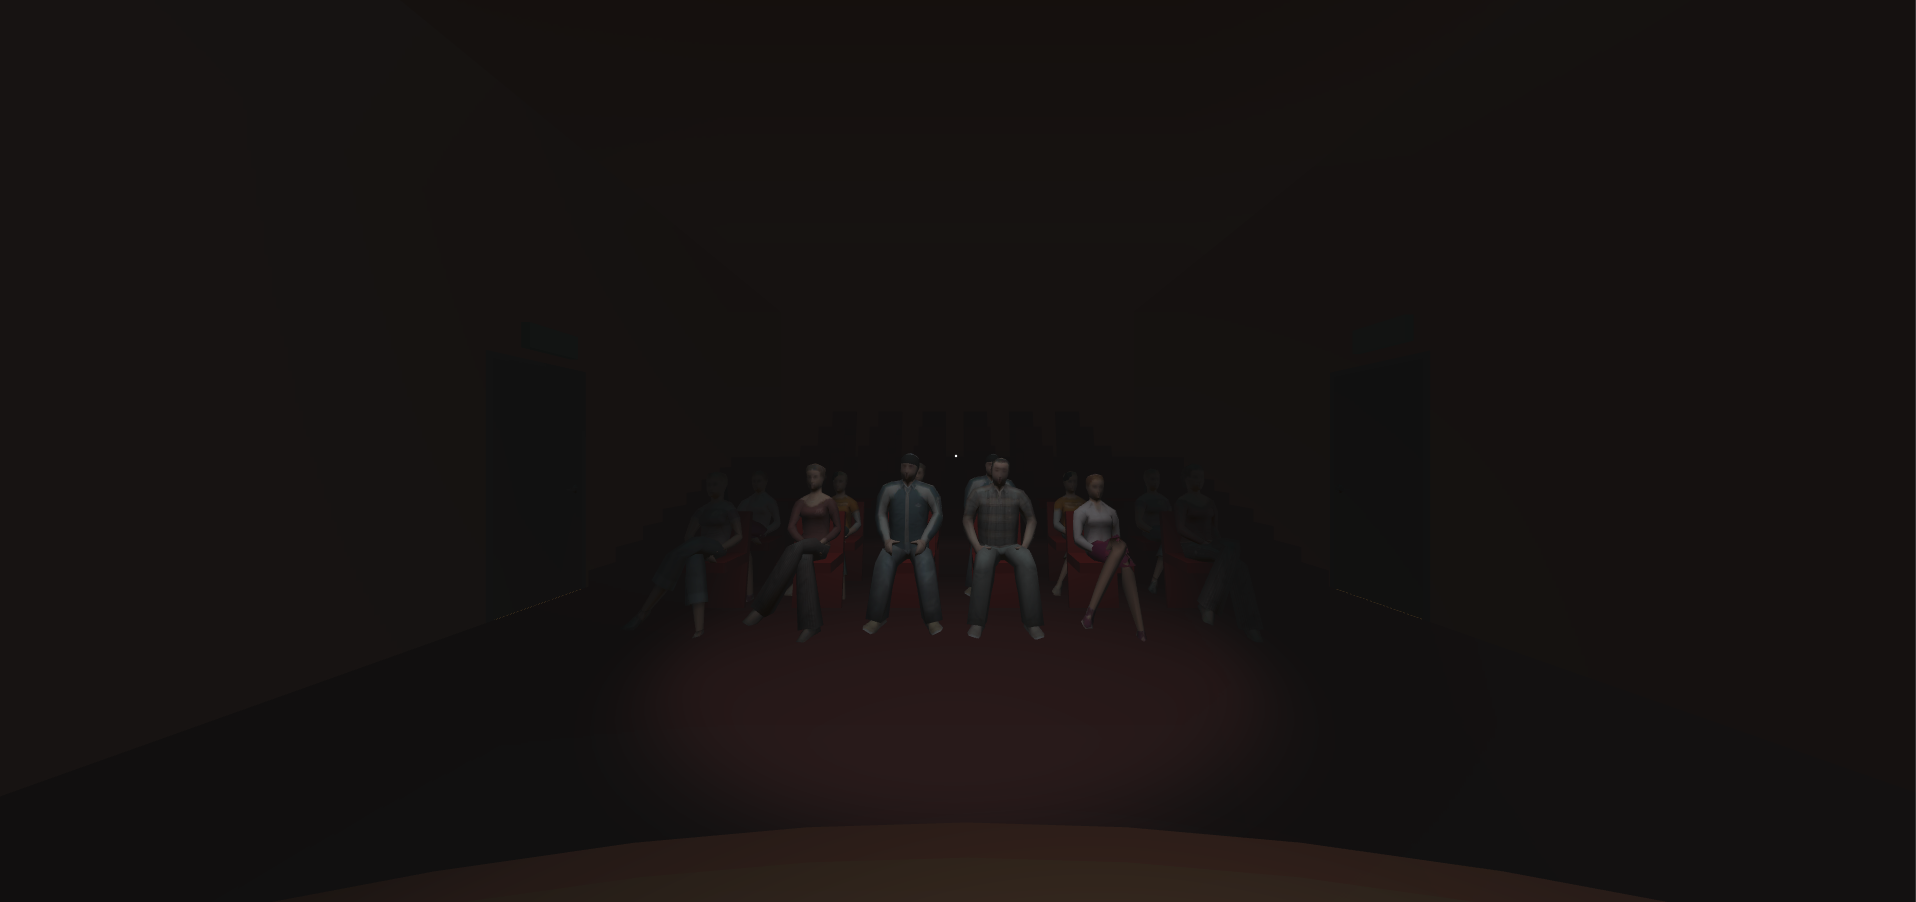
\includegraphics[scale=0.20]{Screenshot}
	\caption{Stage 3: VR activity}
\end{figure}
\subsection{Scenario}
\subsubsection{Scenario 1}
Paolo has been working on a project for a course at the university. He has to present it to the professors at the end of the semester together with his teammate Roberto. He is really nervous about it and so it decides to try a new application he found recently. Paolo asks Roberto to help him coming up with possible questions that the professor could ask. Paolo puts on the Empatica E4 on his wrist and connect it to Roberto's phone and he starts the main application on his smartphone. He then follows the instruction: he scans the QR code that appears on Roberto's phone, selects the interview mode and then selects the easy difficulty without changing the suggested value.\\
He puts on the HMD on and starts with the first activity suggested to him. When the activity finishes, he starts answering the questions that Roberto sent.  

\subsubsection{Scenario 2}
Giulia has to hold a speech in front of an audience for an important event and she is really afraid to not be able to do it correctly. A new application that came out recently was suggested to her by her friend to try her speech and see how well it goes.\\
He decides to follow the suggestion, and so she downloads the app, she puts on the Empatica E4 and follows the instruction on screen: she scan the QR code, she select Solo mode and select the easy difficulty but still change some of the preset values.
She puts on the HMD on and starts with the first activity. When it finishes, she starts her speech.